\documentclass[titlepage, letterpaper, fleqn]{article}
\usepackage[utf8]{inputenc}
\usepackage{fancyhdr} % fancy headers, of course!
\usepackage{amsmath} % what do you think?
\usepackage{amsthm} % theorems!
\usepackage{extramarks} % more cute things
\usepackage{enumitem} % i'm not sure...
\usepackage{multicol} % multicolumn...?
\usepackage{amssymb} % more symbols
\usepackage{MnSymbol} % moar symbols?
\usepackage{booktabs} % cool looking tables
\usepackage{tikz} %venn and shizzle
\usepackage{tikz-qtree-compat} %tableaux
\usepackage{lipsum} %lorem ipsum dolor sit amet f u
\usepackage{mathrsfs} %math script for calligraphic scripting, I GUESS

\topmargin=-0.45in
\evensidemargin=0in
\oddsidemargin=0in
\textwidth=6.5in
\textheight=9.0in
\headsep=0.25in


%
% You should change this things~
%

\newcommand{\mahteacher}{Dr. Viacheslav Kalashnikov}
\newcommand{\mahclass}{Applied Mathematics}
\newcommand{\mahtitle}{Topic IV - Activity 18}
\newcommand{\mahdate}{November 16, 2016}
\newcommand{\spacepls}{\vspace{5mm}}
\newcommand{\until}{\mathscr{U}}
\renewcommand\qedsymbol{\(\blacksquare\)}

%
% Header markings
%

\pagestyle{fancy}
\lhead{1170065 - Xavier Sánchez}
\chead{}
\rhead{}
\lfoot{}
\rfoot{}


\renewcommand\headrulewidth{0.4pt}
\renewcommand\footrulewidth{0.4pt}

\setlength\parindent{0pt}


%
% Create Problem Sections (stolen directly from jdavis/latex-homework-template @ github!)
%

\newcommand{\enterProblemHeader}[1]{
\nobreak\extramarks{}{Problem \arabic{#1} continued on next page\ldots}\nobreak{}
\nobreak\extramarks{Problem \arabic{#1} (continued)}{Problem \arabic{#1} continued on next page\ldots}\nobreak{}
}

\newcommand{\exitProblemHeader}[1]{
\nobreak\extramarks{Problem \arabic{#1} (continued)}{Problem \arabic{#1} continued on next page\ldots}\nobreak{}
\stepcounter{#1}
\nobreak\extramarks{Problem \arabic{#1}}{}\nobreak{}
}

\setcounter{secnumdepth}{0}
\newcounter{partCounter}
\newcounter{homeworkProblemCounter}
\setcounter{homeworkProblemCounter}{1}
\nobreak\extramarks{Exercise \arabic{homeworkProblemCounter}}{}\nobreak{}

%Solution Environment
\newenvironment{solution}
{\renewcommand\qedsymbol{$\square$}\begin{proof}[Solution]}
{\end{proof}}

% Alias for the Solution section header
%\newcommand{\solution}{\textbf{\Large Solution}}

%Alias for the new step section
\newcommand{\steppy}[1]{\textbf{\large #1}}

%
% Homework Problem Environment
%
% This environment takes an optional argument. When given, it will adjust the
% problem counter. This is useful for when the problems given for your
% assignment aren't sequential. See the last 3 problems of this template for an
% example.
%
\newenvironment{homeworkProblem}[1][-1]{
\ifnum#1>0
\setcounter{homeworkProblemCounter}{#1}
\fi
\section{Exercise \arabic{homeworkProblemCounter}}
\setcounter{partCounter}{1}
\enterProblemHeader{homeworkProblemCounter}
}{
\exitProblemHeader{homeworkProblemCounter}
}

%
% My actual info
%

\title{
\vspace{1in}
\textbf{Tecnológico de Monterrey} \\
\vspace{0.5in}
\textmd{\mahclass} \\
\large{\textit{\mahteacher}} \\
\vspace{0.5in}
\textsc{\mahtitle}\\
\textsc{Sample Frequency, Mean, Variance and Standard Deviation}\\
\textsc{4.1.1}\\
\textsc{4.1.2}\\
\textsc{4.1.3}\\
\author{01170065  - MIT \\
Xavier Fernando Cuauhtémoc Sánchez Díaz \\
\texttt{xavier.sanchezdz@gmail.com}}
\date{\mahdate}
}

\begin{document}

\begin{titlepage}
\maketitle
\end{titlepage}

%
% Actual document starts here~
%

\section{Exercise 4.1.1}

{\large The following is a sample of prices, rounded to the nearest cent, charged per gallon of standard unleaded gasoline in the San Francisco Bay area in June 1997.

137, 139, 141, 137, 144, 141, 139, 137, 144, 141, 143, 143, 141.

Represent these data in a frequency table and a relative frequency line graph.}

\begin{table}[h!]
\centering
\begin{tabular}{@{}cc@{}}
\toprule
Price & Frequency \\ \midrule
137   & 3         \\
139   & 2         \\
141   & 4         \\
143   & 2         \\
144   & 2         \\ \bottomrule
\end{tabular}
\caption{Price per gallon of gasoline in SF Bay area}
\label{tab:4.1.1}
\end{table}

\spacepls

\begin{figure}[h!]
	\centering
	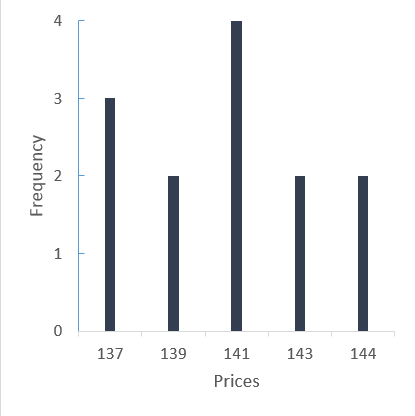
\includegraphics[width=0.3\textwidth]{img_4_1_1}
	\caption{Relative frequency line graph of Table \ref{tab:4.1.1}}
	\label{fig:4.1.1}
\end{figure}

\section{Exercise 4.1.2}

{\large The following are the percentages of ash content in 12 samples of coal found in close proximity:

9.2, 14.1, 9.8, 12.4, 16.0, 12.6, 22.7, 18.9, 21.0, 14.5, 20.4, 16.9

Find the sample mean and sample standard deviation of these percentages.}

\begin{solution}
The sample mean is calculated as the average, and it's approximately 15.7083.

The standard deviation is calculated as the square root of the variance.
The variance is calculated as $\frac{1}{n-1}\sum_{i=1}^{n} (x_i - x)^2$.
The variance of these data is approximately 19.31902,
and therefore the standard deviation is approximately 4.39534.
\end{solution}

\pagebreak

\section{Exercise 4.1.3}

{\large The following data represent the lifetimes (in hours) of a sample of 40 transistors:

112, 121, 126, 108, 141, 104, 136, 134,
121, 118, 143, 116, 108, 122, 127, 140,
113, 117, 126, 130, 134, 120, 131, 133,
118, 125, 151, 147, 137, 140, 132, 119,
110, 124, 132, 152, 135, 130, 136, 128

Determine the sample mean, median and mode, and give a cumulative relative frequency plot of these data.}

\begin{solution}
The sample mean is obtained as the average of all elements, that is $\dfrac{\sum_{i=0}^{i=40}x}{40} = 127.425$.

Since there are 40 elements, then the median is obtained as the average of the $\frac{n}{2}$-th and $\frac{n}{2} + 1$-th elements when ordered.
Therefore, the median is 127.5.

The mode is the most recurring value.
Since there are many recurring values in the array of data, then there are several modal values.
These are 108, 118, 121, 126, 130, 132, 134, 136, 140.

\begin{figure}[h!]
	\centering
	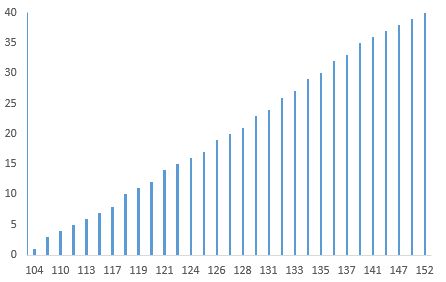
\includegraphics[width=0.5\textwidth]{img_4_1_3}
	\caption{Cumulative relative frequency plot of transistor lifetimes}
	\label{fig:4.1.3}
\end{figure}
\end{solution}

\end{document}